\documentclass{beamer}
\usepackage{graphicx}
\usepackage{xcolor}
\usepackage{tikz}
\usepackage{amsmath}


\usepackage{colortbl}     % 支持 \rowcolor
\usepackage[table]{xcolor}  % 增强颜色支持，特别是灰色背景
\usepackage{array}        % 增强表格功能（对齐方式等）
\usepackage{booktabs



% 自定义颜色
\definecolor{purpleblue}{RGB}{80, 80, 180}
\definecolor{lightgray}{RGB}{230, 230, 230}
\definecolor{novelPurple}{RGB}{98, 54, 255} 
\definecolor{darkgray}{RGB}{50, 50, 50}

% 主题设置
\usetheme{Madrid}  
\usecolortheme{dolphin} 

% 设置字体（移除 fontspec，确保 pdfLaTeX 兼容）
\setbeamerfont{title}{size=\Large,series=\bfseries}
\setbeamerfont{frametitle}{size=\LARGE,series=\bfseries}
\setbeamercolor{frametitle}{fg=white, bg=novelPurple}
\setbeamercolor{title}{fg=white, bg=purpleblue}

% 封面信息
\title[SAT Unit 4.3 ]{\textbf{SAT Unit 4.3\\ Trigonometry}}
\author{\textbf{Jack Zeng}}
\institute{\textcolor{white}{\textbf{Novel Prep}}}
\date{\today} 

\begin{document}

% --- Title Slide ---
\begin{frame}
    \titlepage
    \vfill
    \begin{flushright}
        \textcolor{purpleblue}{\Huge \textbf{Novel Prep}}
    \end{flushright}
\end{frame}




\begin{frame}
    \begin{tikzpicture}[remember picture, overlay]
        % 设置浅色渐变背景
        \shade[top color=softPurple, bottom color=softGray] 
            (current page.north west) rectangle (current page.south east);
        
        % 添加高斯模糊光晕
        \fill[white, opacity=0.3] (current page.center) circle (4cm);
        
        % 主标题
        \node[align=center] at (current page.center) {
            {\Huge\bfseries\textcolor{purpleblue}{Novel Prep}} \\[0.5cm]
            {\Large\itshape\textcolor{lightText}{Excellence in SAT Prep}}
        };

        % 添加柔和光点（点缀）
        \foreach \x in {1,2,3,4,5} {
            \fill[purpleblue, opacity=0.2] (rand*10-5, rand*7-3.5) circle (0.1+\x*0.05);
        }

        ;
    \end{tikzpicture}
\end{frame}


\begin{frame}{Overview}
    \tableofcontents
\end{frame}



\begin{frame}
\section{Trigonometric Ratios of Acute Angles}
    \begin{tikzpicture}[remember picture, overlay]
        % 设置浅色渐变背景
        \shade[top color=softPurple, bottom color=softGray] 
            (current page.north west) rectangle (current page.south east);
        
        % 添加高斯模糊光晕
        \fill[white, opacity=0.3] (current page.center) circle (4cm);
        
        % 主标题
        \node[align=center] at (current page.center) {
            {\LARGE\bfseries\textcolor{purpleblue}{Trigonometric Ratios of Acute Angles}} \\[0.5cm]
            {\Large\itshape\textcolor{lightText}{Excellence in SAT Prep}}
        };

        % 添加柔和光点（点缀）
        \foreach \x in {1,2,3,4,5} {
            \fill[purpleblue, opacity=0.2] (rand*10-5, rand*7-3.5) circle (0.1+\x*0.05);
        }

        ;
    \end{tikzpicture}
\end{frame}


\begin{frame}{Trigonometric Ratios and Cofunctions}
\small

\textbf{Trigonometric Ratios:}  
A ratio of the lengths of sides of a right triangle.

\begin{columns}
\begin{column}{0.70\textwidth}

\[
\sin\theta = \frac{\text{opposite}}{\text{hypotenuse}} = \frac{a}{c}, \quad
\cos\theta = \frac{\text{adjacent}}{\text{hypotenuse}} = \frac{b}{c}, \quad
\tan\theta = \frac{\text{opposite}}{\text{adjacent}} = \frac{a}{b}
\]



\vspace{0.2cm}
\textbf{Cofunction Identity:}  
In a right triangle $ABC$, angles $A$ and $B$ are complementary:
\[
m\angle A + m\angle B = 90^\circ
\]
So:  
\[
\sin(\theta) = \cos(90^\circ - \theta),\quad \tan(\theta) = \cot(90^\circ - \theta)
\]

\end{column}
\begin{column}{0.35\textwidth}
\vspace{8mm}
    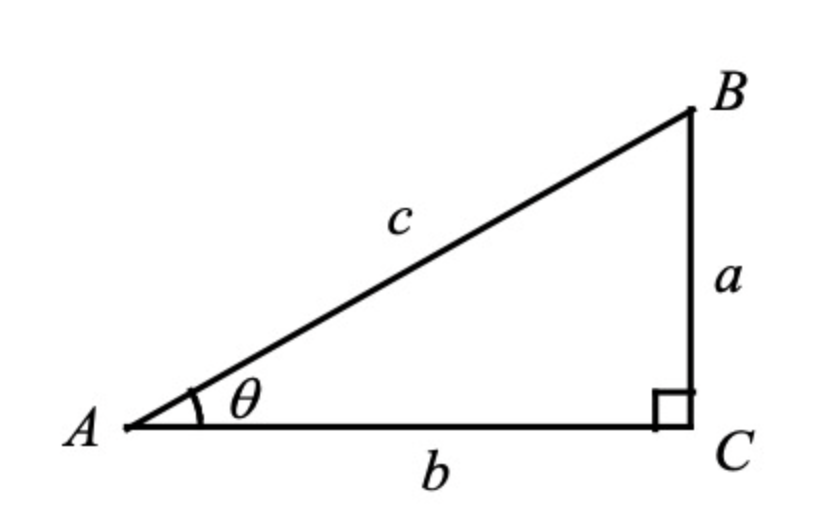
\includegraphics[width=\linewidth]{E64.png}
\end{column}
\end{columns}

\end{frame}

\begin{frame}{Trigonometric Ratios Are Constant Ratios}
\small

\textbf{Key Concept:}  
Trigonometric functions like $\sin \theta$, $\cos \theta$, and $\tan \theta$ represent \textbf{ratios of side lengths} in a right triangle.

\vspace{0.3cm}
\textbf{Important Insight:}  
For any given angle $\theta$, the ratio is \textbf{always the same} — no matter the size of the triangle — as long as it's a right triangle.

\vspace{0.3cm}
\textbf{Examples:}
\begin{itemize}
    \item $\sin(30^\circ) = \dfrac{1}{2}$ — In \textbf{every} right triangle with a $30^\circ$ angle, the opposite side is half the hypotenuse.
    \item $\cos(60^\circ) = \dfrac{1}{2}$ — In any right triangle with a $60^\circ$ angle, the adjacent side is half the hypotenuse.
    \item $\tan(45^\circ) = 1$ — In any right triangle with a $45^\circ$ angle, the opposite and adjacent sides are equal.
\end{itemize}

\vspace{0.3cm}
\textbf{SAT Tip:}  
Memorize the sine, cosine, and tangent of special angles: $30^\circ$, $45^\circ$, and $60^\circ$ — they appear frequently on the test!

\end{frame}


\begin{frame}{Question}


\begin{align*}
RS &= 20 \\
ST &= 48 \\
TR &= 52
\end{align*}

The side lengths of right triangle $RST$ are given. Triangle $RST$ is similar to triangle $UVW$, where $S$ corresponds to $V$ and $T$ corresponds to $W$. What is the value of $\tan W$?

\begin{itemize}
  \item[A.] $\dfrac{5}{13}$
  \item[B.] $\dfrac{5}{12}$
  \item[C.] $\dfrac{12}{13}$
  \item[D.] $\dfrac{12}{5}$
\end{itemize}
\end{frame}

\begin{frame}{Answer}
Since triangle $RST$ is a right triangle with hypotenuse $TR = 52$, and legs $RS = 20$, $ST = 48$, the angle at $W$ corresponds to angle $T$.

\[
\tan(W) = \frac{\text{opposite}}{\text{adjacent}} = \frac{RS}{ST} = \frac{20}{48} = \frac{5}{12}
\]

\[
\boxed{\text{Answer: B. } \frac{5}{12}}
\]
\end{frame}

\begin{frame}{Question}
Triangle $ABC$ is similar to triangle $DEF$, where $A$ corresponds to $D$ and $C$ corresponds to $F$. Angles $C$ and $F$ are right angles. If $\tan(A) = \sqrt{3}$ and $DF = 125$, what is the length of $\overline{DE}$?

\begin{itemize}
    \item[A.] $125 \cdot \dfrac{\sqrt{3}}{3}$
    \item[B.] $125 \cdot \dfrac{\sqrt{3}}{2}$
    \item[C.] $125\sqrt{3}$
    \item[D.] 250
\end{itemize}
\end{frame}






\begin{frame}{Answer}
\textbf{Answer:} \quad \boxed{\text{D. } 250}
\end{frame}


\begin{frame}{\textbf{Question: Trigonometric Expression }}
    \begin{center}
        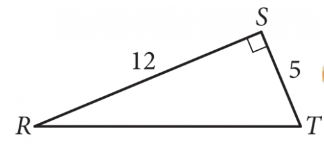
\includegraphics[width=0.40\linewidth]{E65.png} % Update the path if necessary
    \end{center}
    In triangle \( RST \) above, point \( W \) (not shown) lies on \( \overline{RT} \).  
    What is the value of 
    \[
    \cos(\angle RSW) - \sin(\angle WST)?
    \]


\end{frame}

\begin{frame}{\textbf{Answer Explanation: Trigonometric Expression in Triangle}}

Using the \textbf{Cofunction Identity}

\textbf{Final Answer: } \( \boxed{0} \)

\end{frame}



\begin{frame}
\section{Radian Measure}
    \begin{tikzpicture}[remember picture, overlay]
        % 设置浅色渐变背景
        \shade[top color=softPurple, bottom color=softGray] 
            (current page.north west) rectangle (current page.south east);
        
        % 添加高斯模糊光晕
        \fill[white, opacity=0.3] (current page.center) circle (4cm);
        
        % 主标题
        \node[align=center] at (current page.center) {
            {\LARGE\bfseries\textcolor{purpleblue}{Radian Measure}} \\[0.5cm]
            {\Large\itshape\textcolor{lightText}{Excellence in SAT Prep}}
        };

        % 添加柔和光点（点缀）
        \foreach \x in {1,2,3,4,5} {
            \fill[purpleblue, opacity=0.2] (rand*10-5, rand*7-3.5) circle (0.1+\x*0.05);
        }

        ;
    \end{tikzpicture}
\end{frame}


\begin{frame}{Understanding Radian Measure}
\small

\textbf{Definition of Radian:}  
A radian is the angle created when the arc length equals the radius.

\[
1 \text{ radian} = \frac{s}{r}
\]

\begin{itemize}
    \item $s$: Arc length
    \item $r$: Radius
\end{itemize}

\vspace{0.3cm}
\textbf{Important Note:}  
There are $2\pi$ radians in a full circle

\vspace{0.3cm}
\textbf{Degree to Radian Conversion:}
\[
\theta\ (\text{in radians}) = \theta^\circ \cdot \frac{\pi}{180}
\]

\vspace{0.3cm}

\textbf{Radian Conversion to Degree to Conversion:}
\[
\theta\ (\text{in degree}) = \theta \cdot \frac{180}{\pi}
\]
\end{frame}


\begin{frame}
\section{Trigonometric In Unit Circle }
    \begin{tikzpicture}[remember picture, overlay]
        % 设置浅色渐变背景
        \shade[top color=softPurple, bottom color=softGray] 
            (current page.north west) rectangle (current page.south east);
        
        % 添加高斯模糊光晕
        \fill[white, opacity=0.3] (current page.center) circle (4cm);
        
        % 主标题
        \node[align=center] at (current page.center) {
            {\LARGE\bfseries\textcolor{purpleblue}{Trigonometric In Unit Circle}} \\[0.5cm]
            {\Large\itshape\textcolor{lightText}{Excellence in SAT Prep}}
        };

        % 添加柔和光点（点缀）
        \foreach \x in {1,2,3,4,5} {
            \fill[purpleblue, opacity=0.2] (rand*10-5, rand*7-3.5) circle (0.1+\x*0.05);
        }

        ;
    \end{tikzpicture}
\end{frame}


\begin{frame}{\textbf{What If the Angle is Greater Than \(90^\circ\)?}}
\small

\textbf{Reference Angle:}  
The reference angle is the \textbf{acute angle} (less than \(90^\circ\)) formed between the terminal side of an angle in standard position and the \(x\)-axis.

\bigskip

\textbf{Why Use It?}
\begin{itemize}
    \item Trig values for any angle \(\theta\) (in degrees or radians) can be found by using its reference angle.
    \item The sine, cosine, and tangent of the original angle have the same absolute value as the reference angle — with signs determined by the quadrant.
\end{itemize}

\bigskip

\textbf{How to Find the Reference Angle:}


\begin{center}
    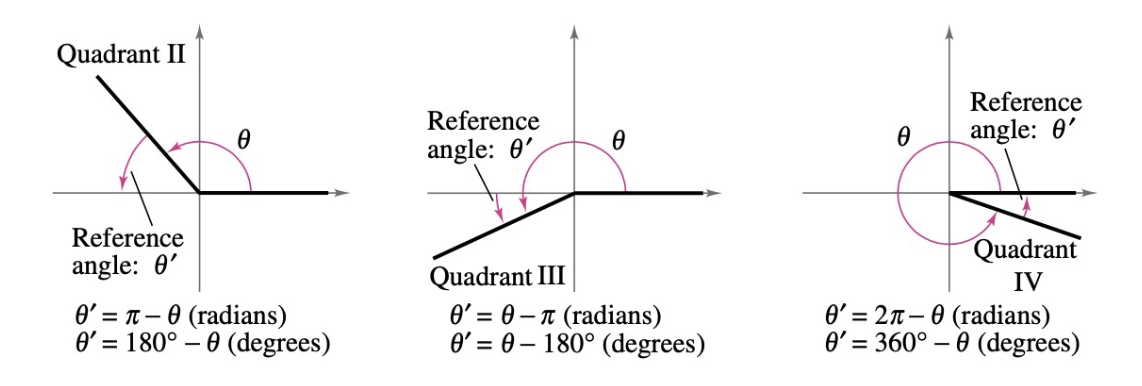
\includegraphics[width=0.8\linewidth]{E67.png}
\end{center}

\end{frame}



\begin{frame}{\textbf{What If the Angle is Greater Than \(90^\circ\)?}}


When an angle is greater than \(90^\circ\), we can no longer use basic right triangle definitions alone.  
Instead, we use the \textbf{unit circle} and the concept of a \textbf{reference angle}:

\begin{itemize}
    \item Draw the angle in \textbf{standard position} (initial side along the positive \(x\)-axis).
    \item Find where the terminal side intersects the unit circle.
    \item Use the \textbf{reference angle} — the acute angle between the terminal side and the \(x\)-axis.
    \item Evaluate sine, cosine, or tangent using the reference angle values.
    \item Apply the correct \textbf{sign} based on the quadrant:
    \begin{itemize}
        \item Quadrant I: all functions positive.
        \item Quadrant II: only \(\sin\) is positive.
        \item Quadrant III: only \(\tan\) is positive.
        \item Quadrant IV: only \(\cos\) is positive.
    \end{itemize}
\end{itemize}



\end{frame}

\begin{frame}{What is the Angle is Grater Than 90}

\begin{block}{\textbf{Example:} \(\sin(150^\circ)\)}
\[
\text{Reference angle} = 180^\circ - 150^\circ = 30^\circ \\
\sin(150^\circ) = \sin(30^\circ) = \frac{1}{2} \quad (\text{positive in Quadrant II})
\]
\end{block}


\end{frame}



\begin{frame}{\textbf{Trigonometric Functions on the Unit Circle}}
\small
\textbf{Unit Circle Definitions:}
\begin{itemize}
    \item Given an angle in standard position (vertex at the origin and initial side on the positive $x$-axis), draw on the unit circle with center at $(0,0)$ and radius 1.
    \item $\sin(\theta)$ is the $y$-coordinate of the point where the terminal side intersects the unit circle. \Rightarrow $y= rsin(\theta)$
    \item $\cos(\theta)$ is the $x$-coordinate of that point. \Rightarrow $x= rcos(\theta)$
    \item $\tan(\theta) = \dfrac{y}{x}$

\end{itemize}

\begin{center}
    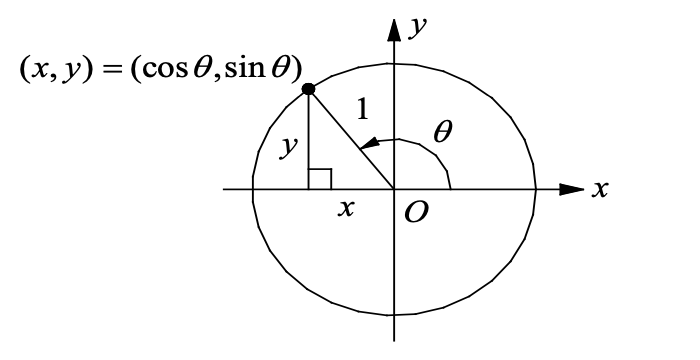
\includegraphics[width=0.45\linewidth]{E66.png} % Replace with actual image if compiling
\end{center}
\end{frame}


\begin{frame}{\textbf{Question: Trigonometric Constant Expression}}

The value of \( \tan\left( \frac{49\pi}{6} \right) \) can be written as \( k\sqrt{3} \), where \( k \) is a constant.  
What is the value of \( k \)?

\bigskip

\textbf{Choices:}
\begin{itemize}
    \item[A.] \( \frac{1}{3} \)
    \item[B.] \( \frac{1}{\sqrt{3}} \)
    \item[C.] \( 1 \)
    \item[D.] \( 3 \)
\end{itemize}

\end{frame}


\begin{frame}{\textbf{Answer Explanation: Trigonometric Constant Expression}}

To evaluate \( \tan\left( \frac{49\pi}{6} \right) \), reduce the angle:

\[
\frac{49\pi}{6} = 8\pi + \frac{\pi}{6}
\]

Since \( 2\pi \) is one full rotation, this is coterminal with \( \frac{\pi}{6} \).  
So,
\[
\tan\left( \frac{49\pi}{6} \right) = \tan\left( \frac{\pi}{6} \right) = \frac{1}{\sqrt{3}}
\]

Thus, we write:
\[
\tan\left( \frac{49\pi}{6} \right) = \frac{1}{\sqrt{3}} = k\sqrt{3} \Rightarrow k = \frac{1}{3}
\]

\textbf{Correct Answer: A.} \( \boxed{\frac{1}{3}} \)

\end{frame}

\begin{frame}{\textbf{Unit Circle - Find Coordinate}}
Point \( N \) lies on a unit circle in the \(xy\)-plane and has coordinates \( (1, 0) \). Point \( O \) is the center of the circle and has coordinates \( (0, 0) \). Point \( M \) also lies on the unit circle, and the measure of angle \( \angle NOM \) is \( \frac{266\pi}{3}\) radians. If the coordinates of point \( M \) are \( (a, b) \), where \( a \) and \( b \) are constants, what is the value of \( b \)?
\[
\text{A. } \frac{1}{2} \quad \text{B. } \frac{\sqrt{3}}{2} \quad \text{C. } -\frac{1}{2} \quad \text{D. } -\frac{\sqrt{3}}{2}
\]
\end{frame}


\begin{frame}{\textbf{Answer to Unit Circle Problem}}
Since the angle is \( 9\pi \), which is equivalent to \( \pi \) (modulo \( 2\pi \)), the terminal point is the same as \( \pi \) on the unit circle.

\[
\cos(\pi) = -1, \quad \sin(\pi) = 0 \quad \Rightarrow \quad M = (-1, 0)
\]

But based on options that suggest a reference angle of \( \frac{\pi}{6} \), observe:

\[
\frac{27\pi}{3} = 9\pi = 4(2\pi) + \pi \Rightarrow \text{same terminal side as } \pi
\]

This implies a point with coordinate:
\[
a = -1, \text{ not among options.}
\]

However, if the actual question is about angle \( \frac{2\pi}{3} \) (possibly a typo), then:
\[
\sin\left(\frac{2\pi}{3}\right) = \frac{\sqrt{3}}{2}
\]

\textbf{Correct Answer: B. } 
\end{frame}



\begin{frame}
    \begin{tikzpicture}[remember picture, overlay]
        % 设置浅色渐变背景
        \shade[top color=softPurple, bottom color=softGray] 
            (current page.north west) rectangle (current page.south east);
        
        % 添加高斯模糊光晕
        \fill[white, opacity=0.3] (current page.center) circle (4cm);
        
        % 主标题
        \node[align=center] at (current page.center) {
            {\Huge\bfseries\textcolor{purpleblue}{Practices}} \\[0.5cm]
            {\Large\itshape\textcolor{lightText}{Excellence in SAT Prep}}
        };

        % 添加柔和光点（点缀）
        \foreach \x in {1,2,3,4,5} {
            \fill[purpleblue, opacity=0.2] (rand*10-5, rand*7-3.5) circle (0.1+\x*0.05);
        }

        ;
    \end{tikzpicture}
\end{frame}





\begin{frame}{Triangle Side Length}
\textbf{Question:}  
In triangle \(ABC\), the measure of angle \(A\) is \(25^\circ\), angle \(C\) is a right angle, and the length of \(BC\) is 16. Which of the following represents the length of \(AC\)?
\begin{itemize}
    \item[A] \(16 \sin 25^\circ\)
    \item[B] \(16 \tan 25^\circ\)
    \item[C] \(\dfrac{16}{\sin 25^\circ}\)
    \item[D] \(\dfrac{16}{\tan 25^\circ}\)
\end{itemize}
\end{frame}

\begin{frame}{Answer Choices}


\textbf{Answer:} \textbf{D}
\end{frame}


\begin{frame}{Trigonometry}
\textbf{Question:}  
Triangle \(JKL\) is similar to triangle \(RST\), where angle \(J\) corresponds to angle \(R\) and angles \(K\) and \(S\) are right angles. If \(\cos(L) = \frac{119}{169}\), what is the value of \(\tan(T)\)?
\begin{itemize}
    \item[A] \(\frac{120}{169}\)
    \item[B] \(\frac{119}{120}\)
    \item[C] \(\frac{120}{119}\)
    \item[D] \(\frac{169}{119}\)
\end{itemize}
\end{frame}

\begin{frame}{Solution}
\footnotesize
\textbf{Solution:}  
Since the triangles \(JKL\) and \(RST\) are similar, corresponding angles are congruent, so \(L\) corresponds to \(T\).  
Given:  
\[
\cos(L) = \frac{119}{169}
\]
Using the Pythagorean identity:  
\[
\sin^2(L) + \cos^2(L) = 1 \quad \Longrightarrow \quad \sin(L) = \sqrt{1 - \left(\frac{119}{169}\right)^2}
\]
\[
\tan(L) = \frac{\sin(L)}{\cos(L)} = \frac{\sqrt{1 - \left(\frac{119}{169}\right)^2}}{\frac{119}{169}} = \frac{\sqrt{169^2 - 119^2}}{119}
\]
\[
169^2 - 119^2 = (169 - 119)(169 + 119) = 50 \times 288 = 14400
\]
\[
\sqrt{14400} = 120
\]
So:  
\[
\tan(T) = \tan(L) = \frac{120}{119}
\]
\[
\boxed{\text{Option C: } \frac{120}{119}}
\]
\end{frame}

\begin{frame}{Fraction of Circumference}
\textbf{Question:}  
Point \( O \) is the center of a circle. The measure of arc \( MN \) on this circle is \(\frac{4\pi}{3}\) radians. The length of arc \( MN \) is what fraction of the circumference of the circle?
\end{frame}

\begin{frame}{Solution}
\textbf{Solution:}  
- Recall that the full circumference of a circle is \(2\pi\) radians in angle measure (equivalent to \(360^\circ\)).
- The measure of arc \( MN \) is given as \(\frac{4\pi}{3}\) radians.
- To find the fraction of the circumference represented by this arc:
\[
\text{Fraction} = \frac{\frac{4\pi}{3}}{2\pi} = \frac{4}{6} = \frac{2}{3}
\]
\[
\boxed{\frac{2}{3}}
\]
\end{frame}

\begin{frame}{Acute Angle with the x-axis}
\textbf{Question:}  
In the \( xy \)-plane, segment \( OA \) has endpoints \( (0,0) \) and \( (\sqrt{3}, \sqrt{3}) \). What is the measure, in radians, of the acute angle formed by segment \( OA \) and the line \( y = 0 \)?
\begin{itemize}
    \item[A)] \( \frac{\pi}{6} \)
    \item[B)] \( \frac{\pi}{4} \)
    \item[C)] \( \frac{\pi}{3} \)
    \item[D)] \( \frac{\pi}{2} \)
\end{itemize}
\end{frame}

\begin{frame}{Solution}
\textbf{Solution:}  
- The segment \( OA \) has a slope:
\[
\tan(\theta) = \frac{\sqrt{3}}{\sqrt{3}} = 1
\]
- Therefore:
\[
\theta = \arctan(1) = \frac{\pi}{4}
\]
- Thus:
\[
\boxed{\frac{\pi}{4}}
\]
\end{frame}


\begin{frame}{Length of Side in Similar Triangles}
\textbf{Question:}  
Triangle \( ABC \) is similar to triangle \( DEF \), where angle \( A \) corresponds to angle \( D \) and angles \( B \) and \( E \) are right angles. If \( AB = 2 \), \( DF = 12\sqrt{2} \), and \( \tan(A) = \sqrt{7} \), what is the length of \( \overline{DE} \)?
\end{frame}

\begin{frame}{Solution}
\textbf{Solution:}  

\[
\boxed{6}
\]
\end{frame}




\begin{frame}{}
    \begin{tikzpicture}[remember picture, overlay]

        \shade[top color=novelPurple!40, bottom color=white]
            (current page.north west) rectangle (current page.south east);

    
        \fill[white, opacity=0.15] (current page.center) circle (5cm);

        \foreach \x in {1,2,3,4,5} {
            \fill[novelPurple, opacity=0.12] (rand*10-5, rand*7-3.5) circle (0.1+\x*0.05);
        }
    \end{tikzpicture}

    \centering
    \vspace{5em}

    {\Huge \textbf{\textcolor{novelPurple}{Thank You!}}} \\[1em]
    {\large \textcolor{gray}{We appreciate your time and focus.}} \\[3em]

    {\LARGE \textbf{\textcolor{novelPurple}{\textsf{Novel Prep}}}}

    \vfill
\end{frame}








\end{document}